\documentclass[14pt]{extbook}
\usepackage{multicol, enumerate, enumitem, hyperref, color, soul, setspace, parskip, fancyhdr} %General Packages
\usepackage{amssymb, amsthm, amsmath, latexsym, units, mathtools} %Math Packages
\everymath{\displaystyle} %All math in Display Style
% Packages with additional options
\usepackage[headsep=0.5cm,headheight=12pt, left=1 in,right= 1 in,top= 1 in,bottom= 1 in]{geometry}
\usepackage[usenames,dvipsnames]{xcolor}
\usepackage{dashrule}  % Package to use the command below to create lines between items
\newcommand{\litem}[1]{\item#1\hspace*{-1cm}\rule{\textwidth}{0.4pt}}
\pagestyle{fancy}
\lhead{Progress Quiz 6}
\chead{}
\rhead{Version C}
\lfoot{4563-7456}
\cfoot{}
\rfoot{Summer C 2021}
\begin{document}

\begin{enumerate}
\litem{
Construct the lowest-degree polynomial given the zeros below. Then, choose the intervals that contain the coefficients of the polynomial in the form $x^3+bx^2+cx+d$.\[ -2 - 5 i \text{ and } 3 \]\begin{enumerate}[label=\Alph*.]
\item \( b \in [-0.9, 3.8], c \in [16, 20.1], \text{ and } d \in [-91, -82] \)
\item \( b \in [-1.5, 0.8], c \in [16, 20.1], \text{ and } d \in [84, 91] \)
\item \( b \in [-0.9, 3.8], c \in [-3.2, -0.5], \text{ and } d \in [-6, -1] \)
\item \( b \in [-0.9, 3.8], c \in [0.2, 7.4], \text{ and } d \in [-15, -11] \)
\item \( \text{None of the above.} \)

\end{enumerate} }
\litem{
Which of the following equations \textit{could} be of the graph presented below?
\begin{center}
    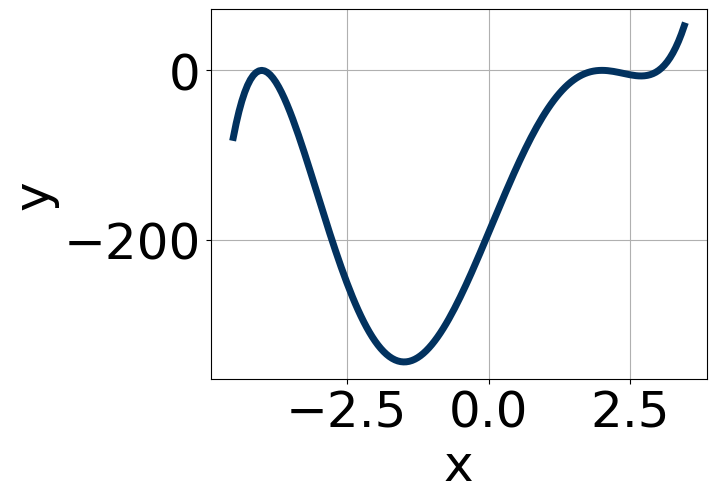
\includegraphics[width=0.5\textwidth]{../Figures/polyGraphToFunctionC.png}
\end{center}
\begin{enumerate}[label=\Alph*.]
\item \( 13(x + 4)^{6} (x - 2)^{5} (x - 3)^{9} \)
\item \( -18(x + 4)^{4} (x - 2)^{10} (x - 3)^{6} \)
\item \( 8(x + 4)^{6} (x - 2)^{8} (x - 3)^{9} \)
\item \( 3(x + 4)^{8} (x - 2)^{9} (x - 3)^{4} \)
\item \( -8(x + 4)^{4} (x - 2)^{8} (x - 3)^{5} \)

\end{enumerate} }
\litem{
Which of the following equations \textit{could} be of the graph presented below?
\begin{center}
    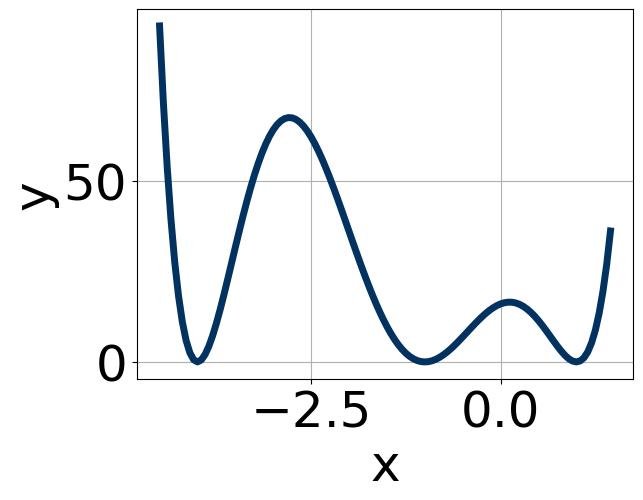
\includegraphics[width=0.5\textwidth]{../Figures/polyGraphToFunctionCopyC.png}
\end{center}
\begin{enumerate}[label=\Alph*.]
\item \( -18(x + 4)^{10} (x + 1)^{4} (x - 1)^{8} \)
\item \( 20(x + 4)^{8} (x + 1)^{5} (x - 1)^{7} \)
\item \( 18(x + 4)^{6} (x + 1)^{4} (x - 1)^{8} \)
\item \( -4(x + 4)^{10} (x + 1)^{10} (x - 1)^{7} \)
\item \( 6(x + 4)^{8} (x + 1)^{4} (x - 1)^{7} \)

\end{enumerate} }
\litem{
Describe the zero behavior of the zero $x = 6$ of the polynomial below.\[ f(x) = -3(x + 4)^{8}(x - 4)^{5}(x + 6)^{6}(x - 6)^{5} \]\begin{enumerate}[label=\Alph*.]
\begin{multicols}{2}\item 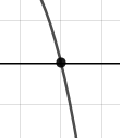
\includegraphics[width = 0.3\textwidth]{../Figures/polyZeroBehaviorCopyAC.png}\item 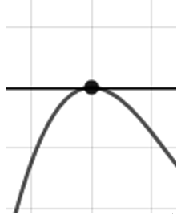
\includegraphics[width = 0.3\textwidth]{../Figures/polyZeroBehaviorCopyBC.png}\item 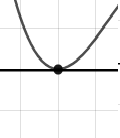
\includegraphics[width = 0.3\textwidth]{../Figures/polyZeroBehaviorCopyCC.png}\item 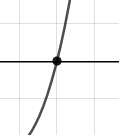
\includegraphics[width = 0.3\textwidth]{../Figures/polyZeroBehaviorCopyDC.png}\end{multicols}\item None of the above.
\end{enumerate} }
\litem{
Construct the lowest-degree polynomial given the zeros below. Then, choose the intervals that contain the coefficients of the polynomial in the form $x^3+bx^2+cx+d$.\[ -2 + 5 i \text{ and } 1 \]\begin{enumerate}[label=\Alph*.]
\item \( b \in [2.3, 3.6], c \in [24, 32], \text{ and } d \in [-30, -20] \)
\item \( b \in [-1.2, 1.7], c \in [-10, -3], \text{ and } d \in [0, 12] \)
\item \( b \in [-1.2, 1.7], c \in [-1, 13], \text{ and } d \in [-5, 0] \)
\item \( b \in [-5.5, -1.7], c \in [24, 32], \text{ and } d \in [23, 32] \)
\item \( \text{None of the above.} \)

\end{enumerate} }
\litem{
Construct the lowest-degree polynomial given the zeros below. Then, choose the intervals that contain the coefficients of the polynomial in the form $ax^3+bx^2+cx+d$.\[ 2, \frac{1}{5}, \text{ and } \frac{-1}{4} \]\begin{enumerate}[label=\Alph*.]
\item \( a \in [17, 29], b \in [-39.3, -36.6], c \in [-5.1, -0.4], \text{ and } d \in [-4, 0] \)
\item \( a \in [17, 29], b \in [47.6, 51.5], c \in [18.7, 20.3], \text{ and } d \in [2, 8] \)
\item \( a \in [17, 29], b \in [-39.3, -36.6], c \in [-5.1, -0.4], \text{ and } d \in [2, 8] \)
\item \( a \in [17, 29], b \in [33.4, 40.5], c \in [-5.1, -0.4], \text{ and } d \in [-4, 0] \)
\item \( a \in [17, 29], b \in [39.7, 41.9], c \in [-2, 2.2], \text{ and } d \in [-4, 0] \)

\end{enumerate} }
\litem{
Describe the end behavior of the polynomial below.\[ f(x) = 5(x - 5)^{4}(x + 5)^{5}(x - 6)^{5}(x + 6)^{6} \]\begin{enumerate}[label=\Alph*.]
\begin{multicols}{2}\item 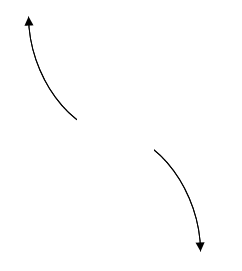
\includegraphics[width = 0.3\textwidth]{../Figures/polyEndBehaviorAC.png}\item 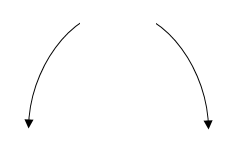
\includegraphics[width = 0.3\textwidth]{../Figures/polyEndBehaviorBC.png}\item 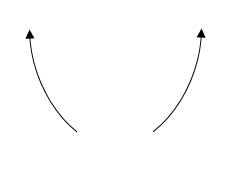
\includegraphics[width = 0.3\textwidth]{../Figures/polyEndBehaviorCC.png}\item 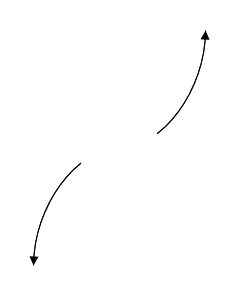
\includegraphics[width = 0.3\textwidth]{../Figures/polyEndBehaviorDC.png}\end{multicols}\item None of the above.
\end{enumerate} }
\litem{
Construct the lowest-degree polynomial given the zeros below. Then, choose the intervals that contain the coefficients of the polynomial in the form $ax^3+bx^2+cx+d$.\[ -5, \frac{-2}{3}, \text{ and } \frac{-7}{5} \]\begin{enumerate}[label=\Alph*.]
\item \( a \in [12, 16], b \in [103, 110], c \in [161, 178], \text{ and } d \in [-74, -62] \)
\item \( a \in [12, 16], b \in [-72, -57], c \in [-75, -65], \text{ and } d \in [68, 74] \)
\item \( a \in [12, 16], b \in [-45, -43], c \in [-142, -136], \text{ and } d \in [-74, -62] \)
\item \( a \in [12, 16], b \in [-113, -105], c \in [161, 178], \text{ and } d \in [-74, -62] \)
\item \( a \in [12, 16], b \in [103, 110], c \in [161, 178], \text{ and } d \in [68, 74] \)

\end{enumerate} }
\litem{
Describe the zero behavior of the zero $x = -9$ of the polynomial below.\[ f(x) = -9(x - 9)^{4}(x + 9)^{5}(x + 3)^{9}(x - 3)^{10} \]\begin{enumerate}[label=\Alph*.]
\begin{multicols}{2}\item 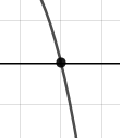
\includegraphics[width = 0.3\textwidth]{../Figures/polyZeroBehaviorAC.png}\item 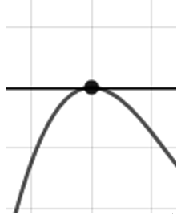
\includegraphics[width = 0.3\textwidth]{../Figures/polyZeroBehaviorBC.png}\item 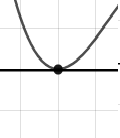
\includegraphics[width = 0.3\textwidth]{../Figures/polyZeroBehaviorCC.png}\item 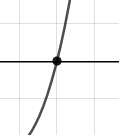
\includegraphics[width = 0.3\textwidth]{../Figures/polyZeroBehaviorDC.png}\end{multicols}\item None of the above.
\end{enumerate} }
\litem{
Describe the end behavior of the polynomial below.\[ f(x) = 5(x - 5)^{5}(x + 5)^{10}(x - 8)^{5}(x + 8)^{7} \]\begin{enumerate}[label=\Alph*.]
\begin{multicols}{2}\item 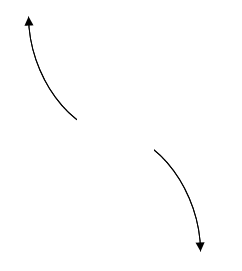
\includegraphics[width = 0.3\textwidth]{../Figures/polyEndBehaviorCopyAC.png}\item 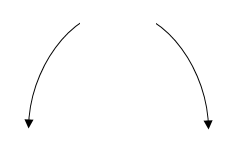
\includegraphics[width = 0.3\textwidth]{../Figures/polyEndBehaviorCopyBC.png}\item 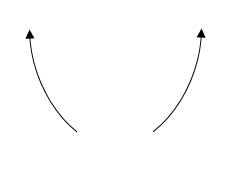
\includegraphics[width = 0.3\textwidth]{../Figures/polyEndBehaviorCopyCC.png}\item 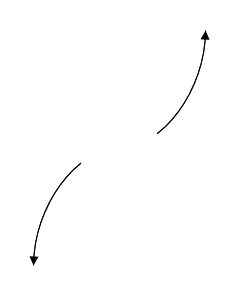
\includegraphics[width = 0.3\textwidth]{../Figures/polyEndBehaviorCopyDC.png}\end{multicols}\item None of the above.
\end{enumerate} }
\end{enumerate}

\end{document}